\documentclass{article}

\usepackage[top=2.54cm, bottom=2.54cm, right=2.54cm, left=2.54cm]{geometry}
\usepackage{graphicx}
\usepackage{xcolor}
\usepackage{hyperref}
\usepackage[font=footnotesize]{caption}
\usepackage[font=scriptsize]{subcaption}
\usepackage{url}
\usepackage{setspace}

\renewcommand{\rmdefault}{phv}
\onehalfspacing

\usepackage{chngcntr}
\counterwithin{figure}{section}

\title{} 
\author{
    Entry Name: \textbf{``LCEE-MC3''}\\
    \textbf{VAST Challenge 2019}\\
    \textbf{\underline{Mini-Challenge 3}}}
\date{}

\begin{document}
%\maketitle

\begin{center}
Entry Name: \textbf{``LCEE-MC3''}\\
\textbf{VAST Challenge 2019}\\
\textbf{\underline{Mini-Challenge 3}}
\end{center}

\noindent
\textbf{Team Members:}\\
Ana Larissa Dias, Federal University of Par\'{a}, \href{mailto:larissa.engcomp@gmail.com}  {\texttt{larissa.engcomp@gmail.com}}   \\
Cassio Batista,   Federal University of Par\'{a}, \href{mailto:cassio.batista.13@gmail.com}{\texttt{cassio.batista.13@gmail.com}} \\
Edwin Rueda,      Federal University of Par\'{a}, \href{mailto:ejrueda95g@gmail.com}       {\texttt{ejrueda95g@gmail.com}}        \\
Erick Campos,     Federal University of Par\'{a}, \href{mailto:erick.c.modesto@gmail.com}  {\texttt{erick.c.modesto@gmail.com}}   \\

\noindent
\textbf{Student Team:} YES \\

\noindent
\textbf{Tools Used:}
\begin{itemize}
    \item \href{https://www.python.org/downloads/}               {Python}           (v3.5.3)
    \item \href{https://bokeh.pydata.org/en/latest/}             {Bokeh}            (v1.2.0)
    \item \href{https://www.nltk.org/}                           {NLTK}             (v3.4.1)
    \item \href{https://textblob.readthedocs.io/}                {TextBlob}         (v0.15.3)
    \item \href{https://www.numpy.org/}                          {NumPy}            (v1.16.0)
    \item \href{https://pandas.pydata.org/}                      {pandas}           (v0.24.2)
    \item \href{https://matplotlib.org/}                         {Matplotlib}       (v3.0.2)
    \item \href{https://github.com/amueller/word_cloud}          {word\_cloud}      (v1.5.0)
    \item \href{https://scikit-learn.org/stable/}                {scikit-learn}     (v0.20.2)
    \item \href{https://nodejs.org/en/download/}                 {Node.js}          (v10.16.0)
    \item \href{https://www.libreoffice.org/}                    {LibreOffice Calc} (v5.2.7.2)
    \item \href{http://man7.org/linux/man-pages/man1/grep.1.html}{grep}             (v2.27)
\end{itemize}

\noindent
\textbf{Approximately how many hours were spent working on this submission in
total?} 168 hours \\

\noindent
\textbf{May we post your submission in the Visual Analytics Benchmark Repository
after VAST Challenge 2019 is complete?} YES \\

\noindent
\textbf{Video:} \url{https://youtu.be/vNlLfvNMXN8}\\

\noindent
\textbf{Questions} \\
\footnotesize{\textcolor{gray}{The City has been using Y*INT to communicate with
its citizens, even post-earthquake. However, City officials needs additional
information to determine the best way to allocate emergency resources across all
neighborhoods of St. Himark. Your task, using your visual analytics on the
community Y*INT data, is to determine the types of problems that are occurring
across the St.  Himark. Then, advise the City on how to prioritize the
distribution of resources. Keep in mind that not all sources on Y*INT are
reliable, and that priorities may change over time as the state of neighborhoods
also changes.}}

\newpage
\begin{enumerate}
    \stepcounter{section}
    \section*{\tiny} % question 1
    \item \textcolor{gray}{Using  visual analytics, characterize conditions
        across the city and recommend how resources should be allocated at 5
        hours and 30 hours after the earthquake. Include evidence from the data
        to support these recommendations. Consider how to allocate resources
        such as road crews, sewer repair crews, power, and rescue teams. 1000
        words, 12 images.}

    In order to discern between reliable and unreliable messages, we have considered
a bar chart of frequency of users that tweeted the most with a hover tool to
show the most frequent words spoken by each user.
Figure~\ref{fig:most_freq_users} shows the unfiltered distribution, in which the
red bars represent users that are probably sellers since their messages include
too many words like ``\emph{deal}'', ``\emph{offer}'', ``\emph{opportunity}'',
``\emph{chances}'', etc. All tweets from those users have therefore been
discarded.

\begin{figure}[!h]
    \centering
    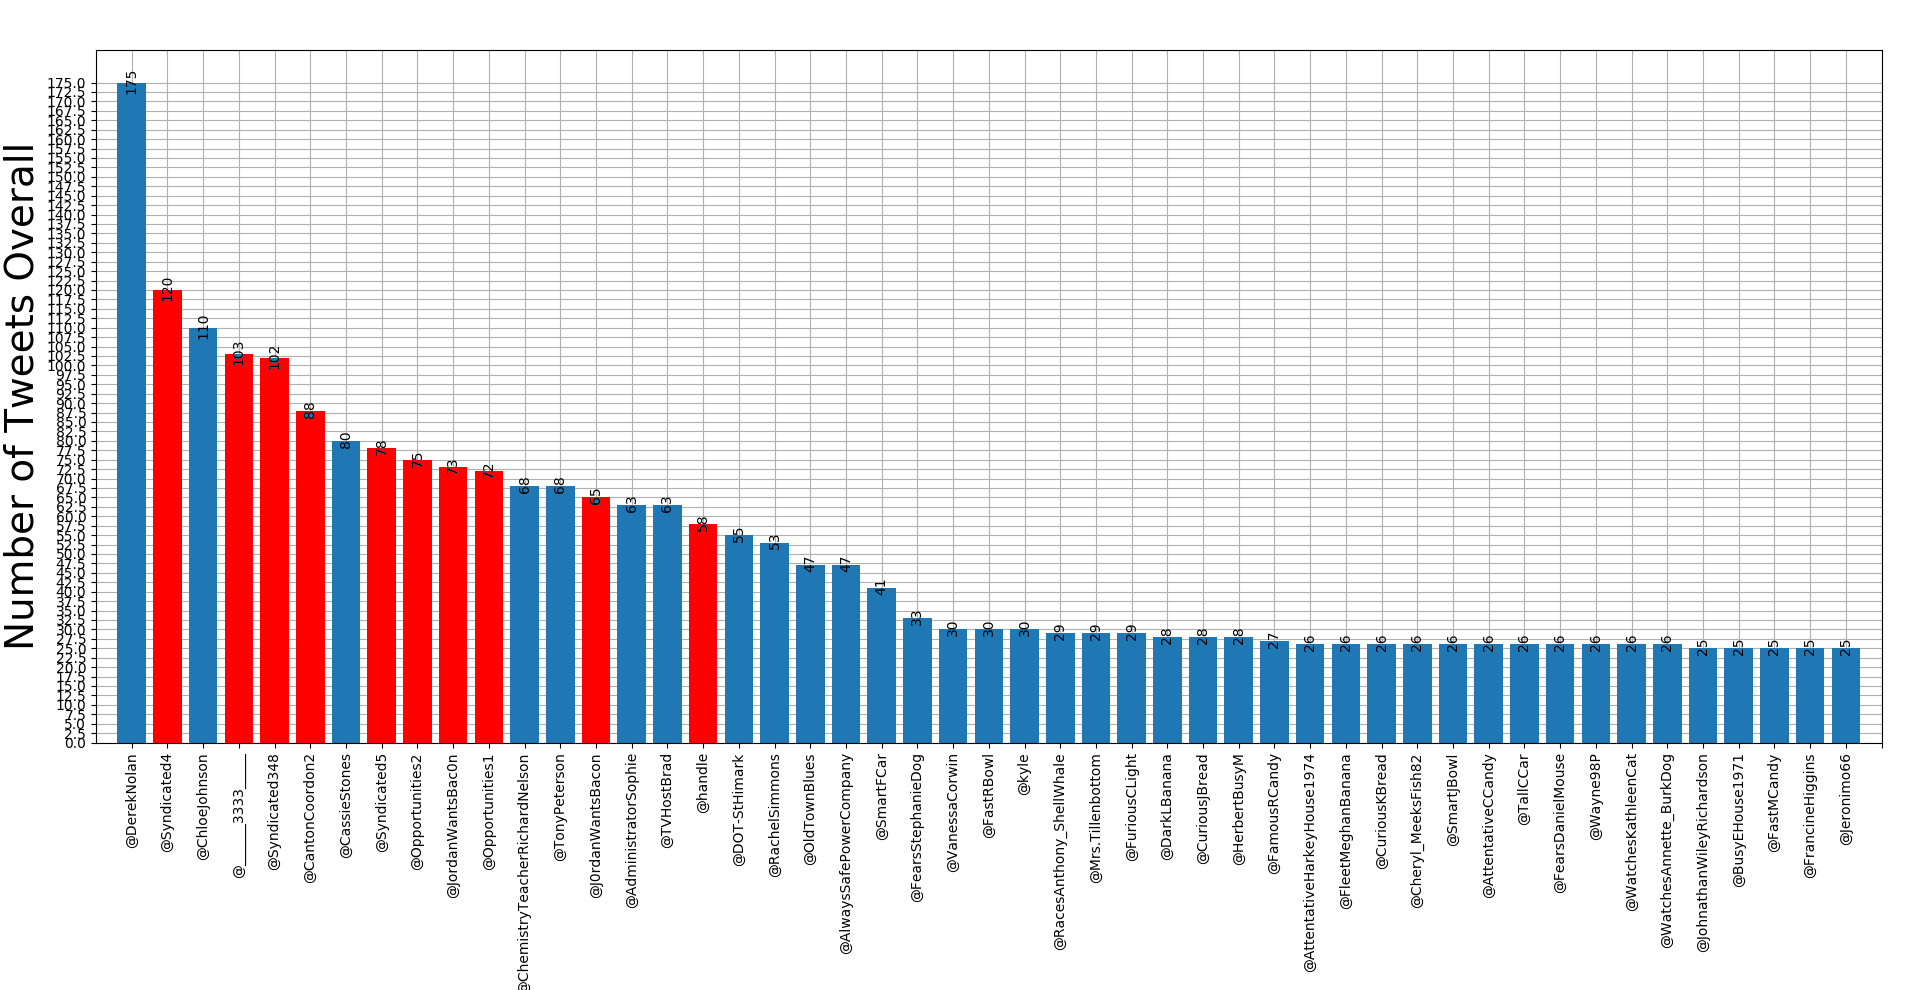
\includegraphics[width=0.95\textwidth]{figs/most_freq_users.png}
    \caption{Most frequent tweeters (usernames). Red bars reresent sellers.}
    \label{fig:most_freq_users}
\end{figure}

There appears to have occurred three earthquakes, but the first one seems to
have started at 2~PM of the first day (April 6th), as
can be seen at the heatmap of Figure~\ref{fig:eq_start_heat}. The heatmap is
divided by a time interval of one hour and by neighbourhood location. It was
generated by considering a list of keywords that were tweeted and are similar in 
meaning (synonyms) and are directly related to the word ``earthquake''. The list 
is: ``\emph{shake}'', ``\emph{shudder}'', ``\emph{vibrate}'', ``\emph{wobble}'',
``\emph{tremor}'', ``\emph{tremble}'', ``\emph{quaver}'', ``\emph{quiver}'',
``\emph{hazard}'', ``\emph{disaster}'', ``\emph{destruction}'', and
``\emph{rubble}''.

\begin{figure}[!h]
    \centering
    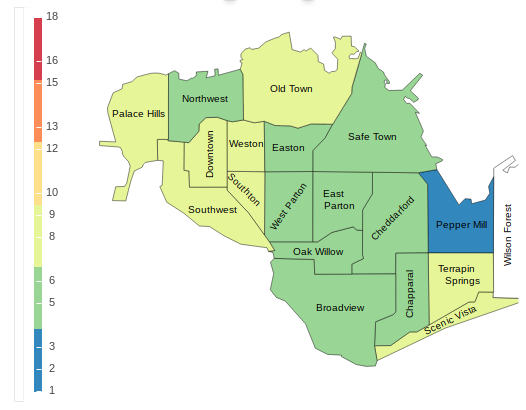
\includegraphics[width=0.50\textwidth]{figs/cond_5h/cond_5h_svg.png}
    \caption{St. Himark's map 5h after the first earthquake. Lighter shades of
    green represent a higher frequency of messages for each location.}
    \label{fig:map_5h}
\end{figure}

To ensure the heatmap is providing a reliable information, a horizontal bar
chart, shown in Figure~\ref{fig:eq_start_hbar}, was used from 1:30~PM to 
3:00~PM. It counts isolated 
words and discards words such as adverbs, pronouns, adjectives, articles and 
some nouns and verbs that were considered to be useless such as ``anyone'',
``make'', ``know'', ``food'', ``hate'', etc. Then the Porter Stemmer from the
\texttt{nltk} package was used to clip the words by its invariant parts (word 
root), and that root was further reduced to 4-chars only. A heat-like colormap
from blue to red was also included to enhance frequency distinction. 

The bar chart shows some interesting other words such as ``\emph{feel}'',
``\emph{hear}'', ``\emph{report}'' apart from the keywords aforementioned, in
which ``\emph{earthquake}'' is the most frequent one in accordance with the red
color.

\begin{figure}[!h]
    \centering
    \begin{subfigure}[!h]{0.95\textwidth}
        \centering
        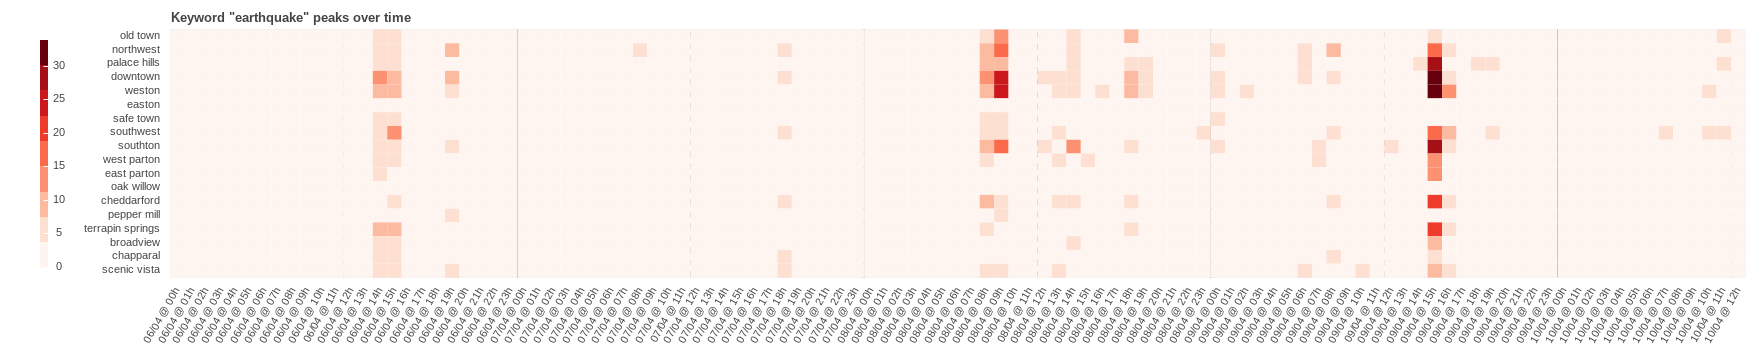
\includegraphics[width=1.00\textwidth]{figs/eq_start_heat.png}
        \caption{Heatmap considering cluster of similar keywords (synonyms)}
        \label{fig:eq_start_heat}
    \vspace{12pt}
    \end{subfigure}
    \begin{subfigure}[!h]{0.95\textwidth}
        \centering
        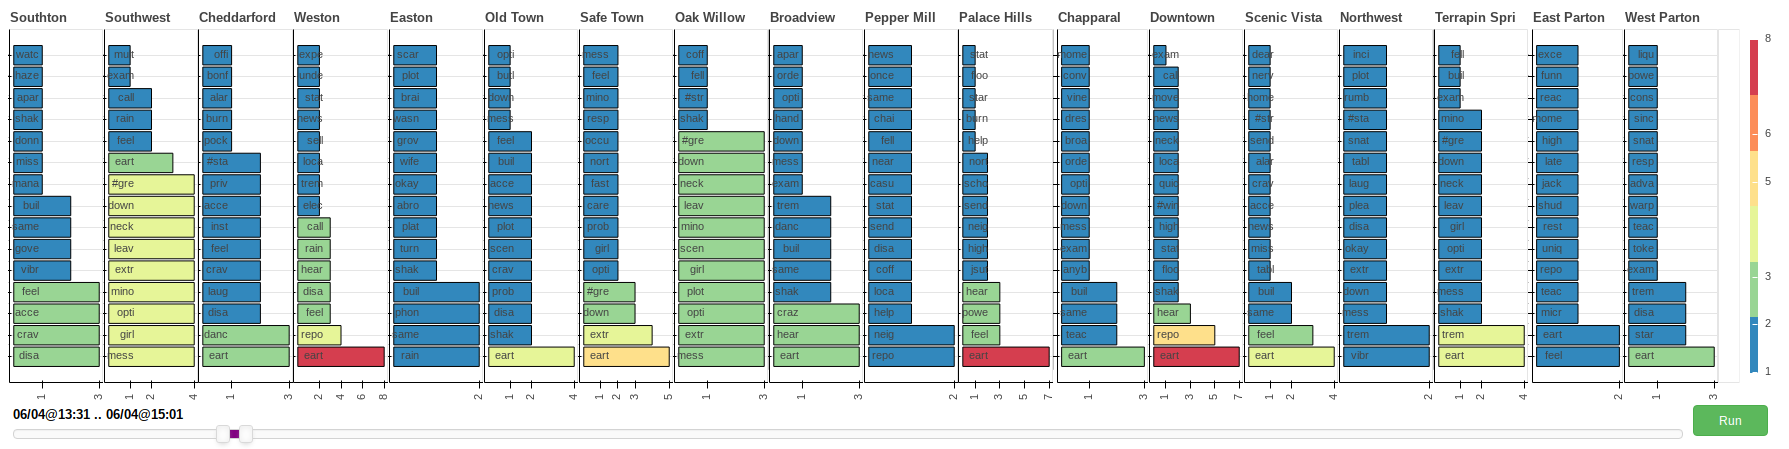
\includegraphics[width=1.00\textwidth]{figs/eq_start_hbar.png}
        \caption{Bar chart with blue-to-red colormap considering frequency of
        words from 1:00~PM to 3~PM of April 6th.}
        \label{fig:eq_start_hbar}
    \end{subfigure}
    \caption{Earthquake start}
    \label{fig:eq_start}
\end{figure}

Figure~\ref{fig:map_5h} shows a dynamically-colored SVG map of the city, where
the neighbourhood inner colors range from blue to red in a heatmap fashion
according to the average mean of the colors of the five bigger bars of the
horizontal bar chart for each location.

Figure~\ref{fig:eq_cond_5h} shows the heatmap per keyword in a five-hour-time 
interval from 2:00~PM to 6:59~PM. The top shows 3 blank graphs for the keywords
``building'', ``medical'', and ``road'', which means these resources do not 
appear to be requested by any neighbourhood. On the other hand, the 3 graphs at
the bottom show the number of mentions for keywords related to 
``sewer and water'' (Figure~\ref{fig:sewer_5h}), 
``power'' (Figure~\ref{fig:power_5h}), and ``rain'' (Figure~\ref{fig:rain_5h}). 

\begin{figure}[!h]
    \centering
    \begin{subfigure}[!h]{0.32\textwidth}
        \centering
        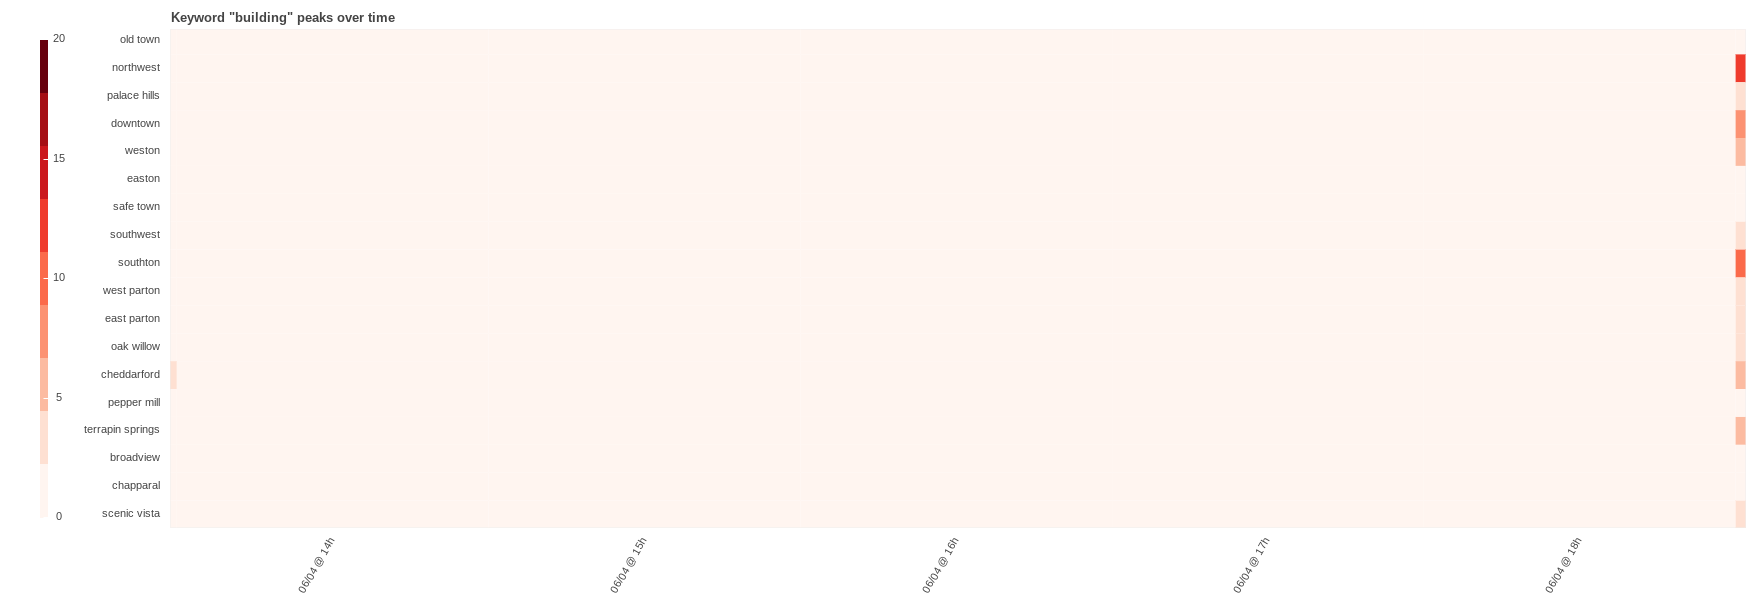
\includegraphics[width=1.00\textwidth]{figs/cond_5h/cond_5h_build.png}
        \caption{Building}
        \label{fig:build_5h}
    \end{subfigure}
    \begin{subfigure}[!h]{0.32\textwidth}
        \centering
        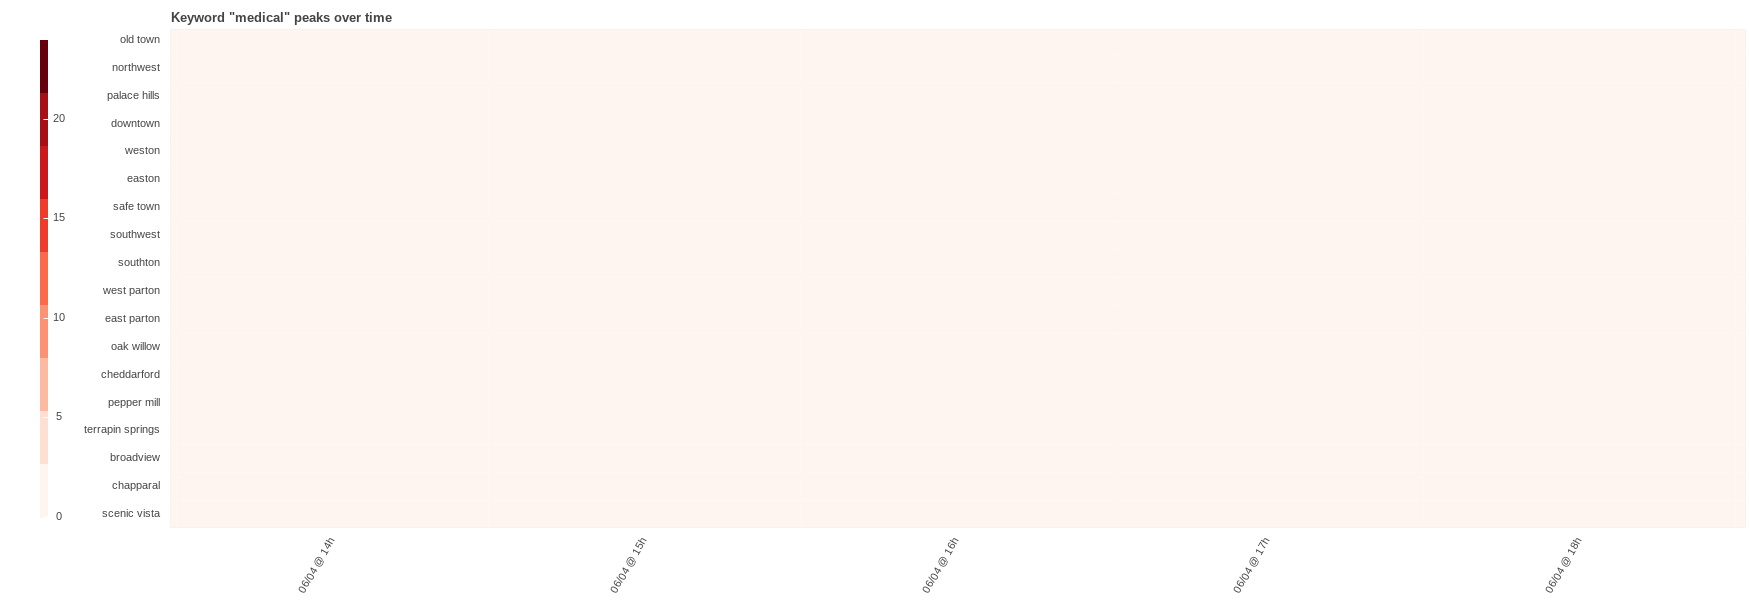
\includegraphics[width=1.00\textwidth]{figs/cond_5h/cond_5h_medical.png}
        \caption{Medical}
        \label{fig:medical_5h}
    \end{subfigure}
    \begin{subfigure}[!h]{0.32\textwidth}
        \centering
        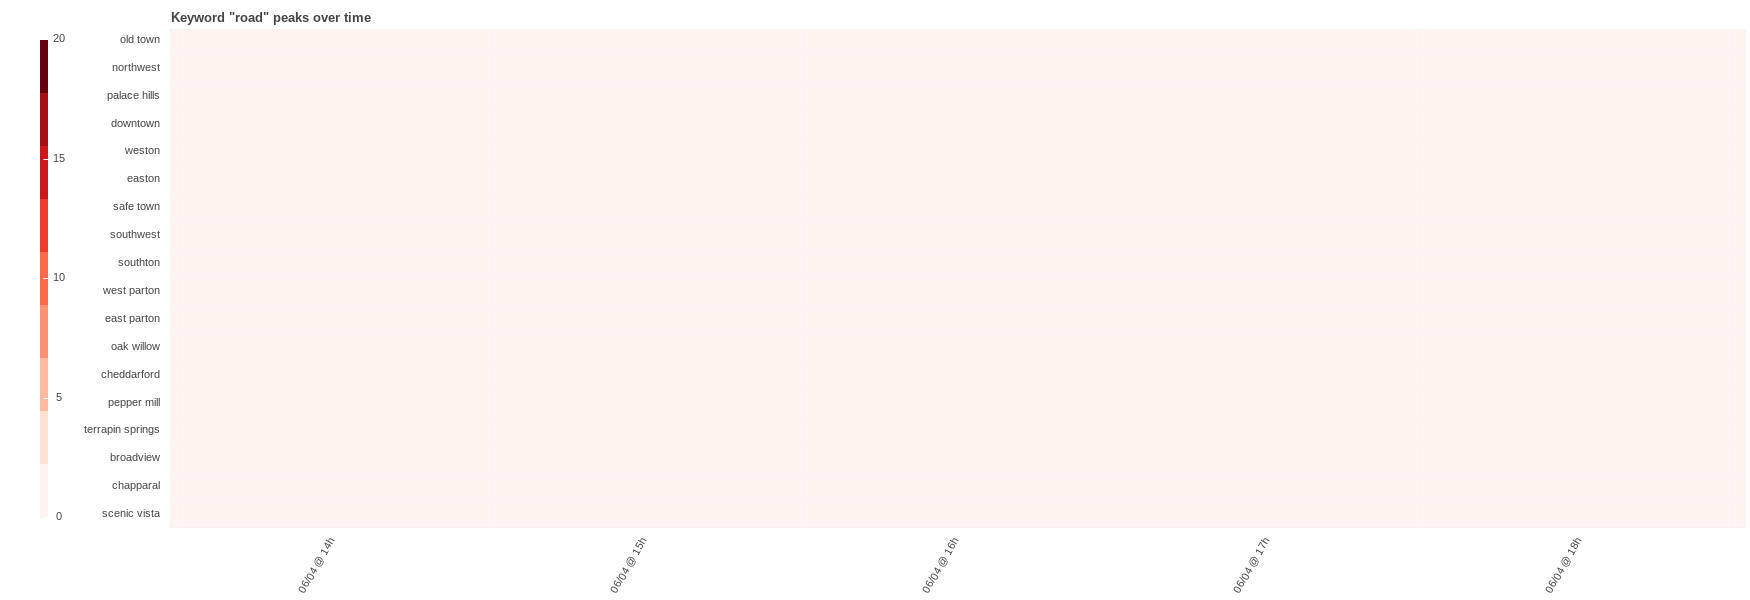
\includegraphics[width=1.00\textwidth]{figs/cond_5h/cond_5h_road.png}
        \caption{Roads and Bridges}
        \label{fig:road_5h}
    \end{subfigure}
    \begin{subfigure}[!h]{0.32\textwidth}
        \centering
        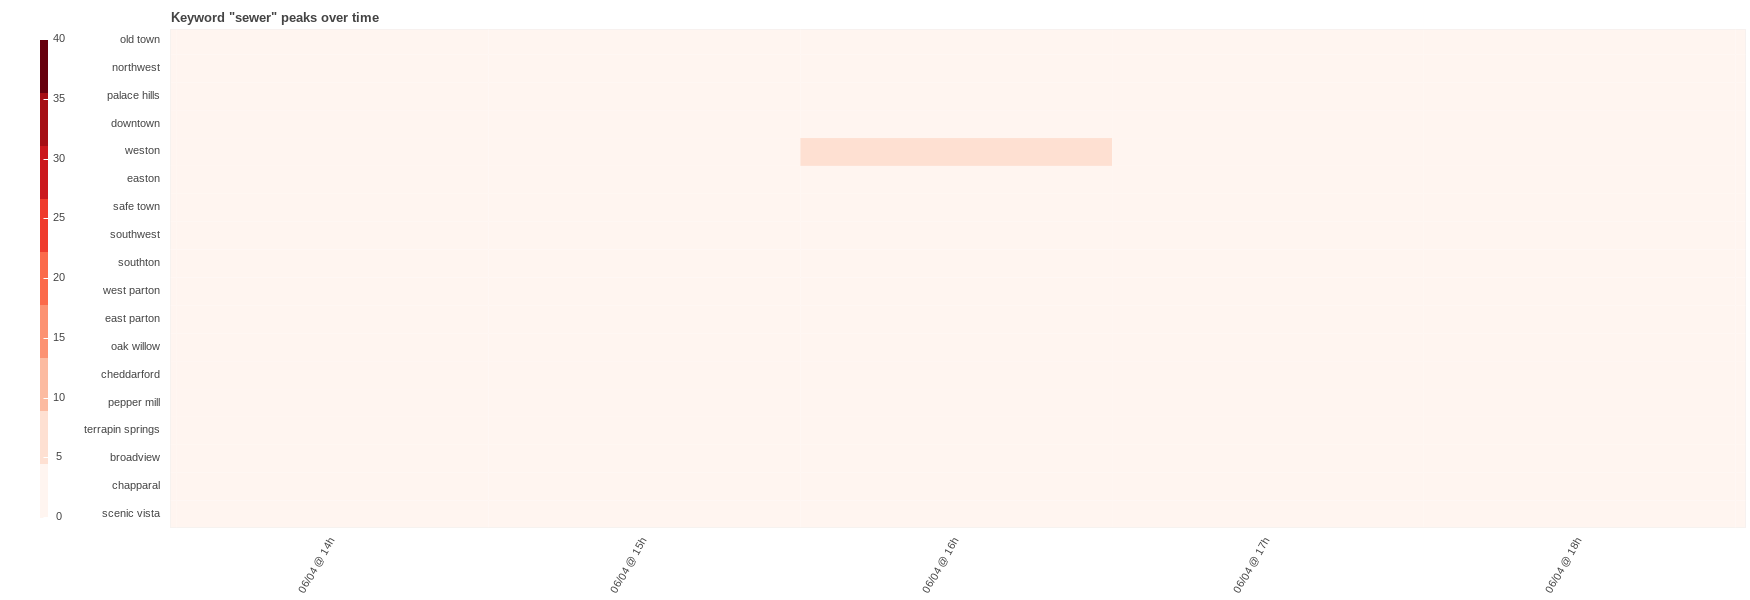
\includegraphics[width=1.00\textwidth]{figs/cond_5h/cond_5h_sewer.png}
        \caption{Sewer and water}
        \label{fig:sewer_5h}
    \end{subfigure}
    \begin{subfigure}[!h]{0.32\textwidth}
        \centering
        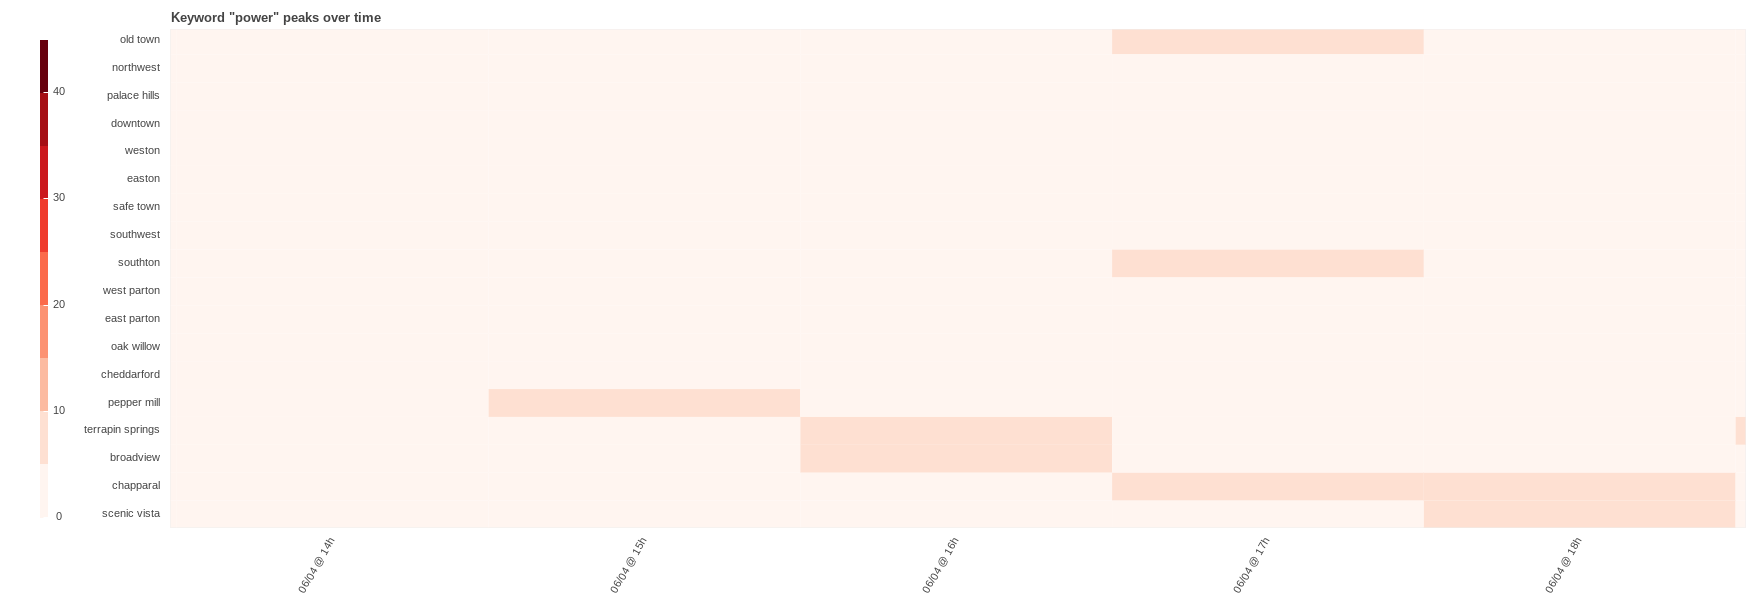
\includegraphics[width=1.00\textwidth]{figs/cond_5h/cond_5h_power.png}
        \caption{Power}
        \label{fig:power_5h}
    \end{subfigure}
    \begin{subfigure}[!h]{0.32\textwidth}
        \centering
        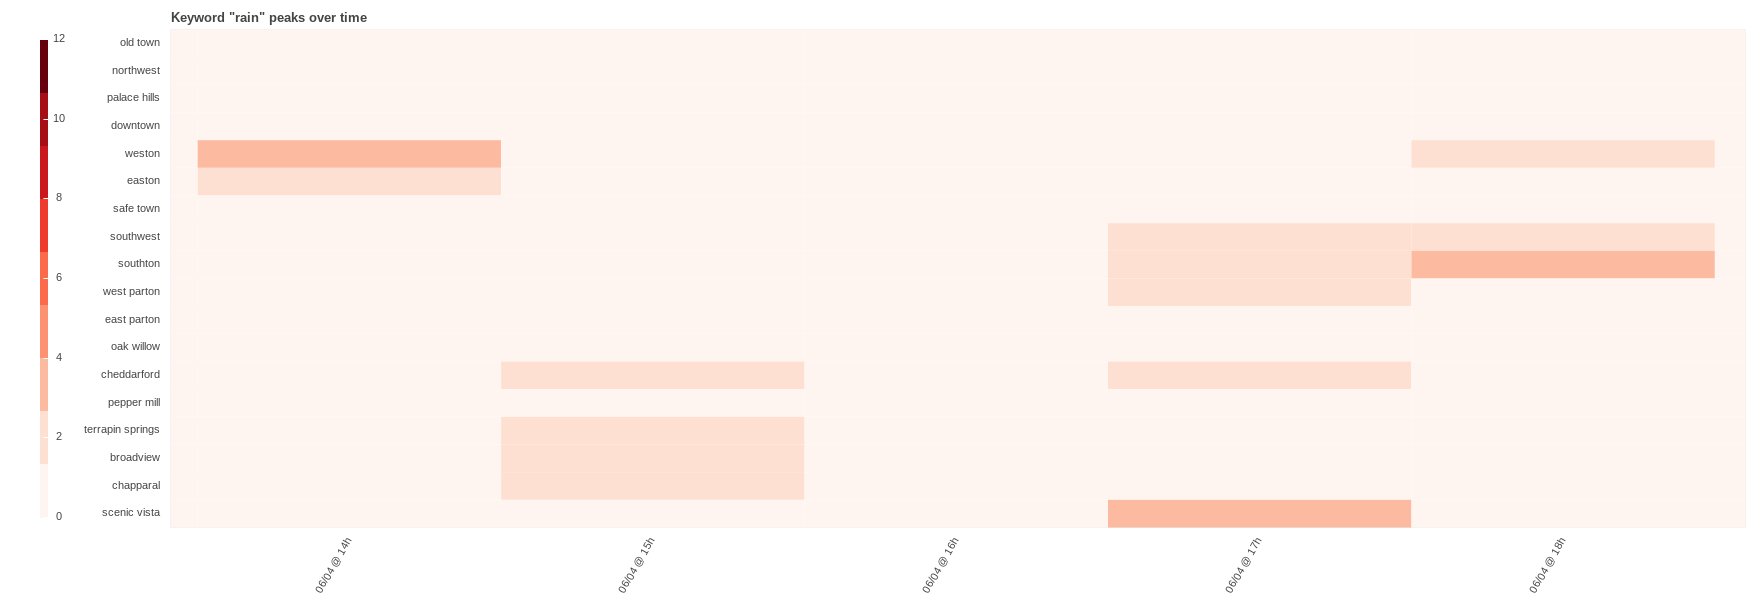
\includegraphics[width=1.00\textwidth]{figs/cond_5h/cond_5h_rain.png}
        \caption{Rain}
        \label{fig:rain_5h}
    \end{subfigure}
    \caption{Conditions after 5h of the first earthquake}
    \label{fig:eq_cond_5h}
\end{figure}

Suggestions for crew allocation is detailed as follows: 

\begin{itemize}
    \item \emph{Sewer and water:} A crew must be sent only to Weston between 
    4:00~PM and 4:59~PM.
    \smallskip 
    \item \emph{Power}: Issues have occurred in Pepper Mill, \textbf{Terrapin
    Springs}, \textbf{Broadview}, Chapparal, \textbf{Southton}, \textbf{Old 
    Town} and Scenic Vista, but we'll consider only the locations 
    highlighted in bold because they have hospitals.
    \begin{itemize}
        \item A crew must be sent to Terrapin Springs between 3:00~PM and
        3:59~PM. Broadview also has a power demand at this time interval but the
        tweet frequency is much lower considering the five-hour period.
        \item Two crews must be sent to Old Town and Southton between 4:00~PM 
        and 4:59~PM.
        \item Lastly, the crew from Terrapin Springs can be reallocated to
        Chapparal between 5:00~PM and 5:59~PM. Although Chapparal does not have
        hospitals, it has been nearly two hours with electrical issues.
    \end{itemize}
    \item \emph{Rescue, sewer and water}: A crew must be sent to Southton only
    because there have been small issues in Weston, Southton and Downtown, and
    therefore Southton is geographically in the middle of such neighbourhoods.
\end{itemize}

%\subsection{How resources should be allocated 30h after the earthquake?}
Looking at the useful-words colormap over the SVG map of St. Hirmak, it can be
inferred right at the outset that the neighbourhoods that are in most need are
Downtown, Southton, Old Town and Weston.

\begin{figure}[!h]
    \centering
    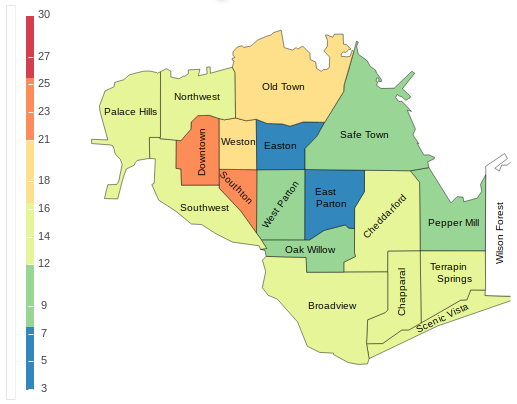
\includegraphics[width=0.50\textwidth]{figs/cond_30h/cond_30h_svg.png}
    \label{fig:map_30h}
    \caption{St. Himark's map 30h after the first earthquake. Yellow and orange 
    shades represent a higher frequency of messages for each location.}
\end{figure}

\begin{figure}[!h]
    \centering
    \begin{subfigure}[!h]{0.24\textwidth}
        \centering
        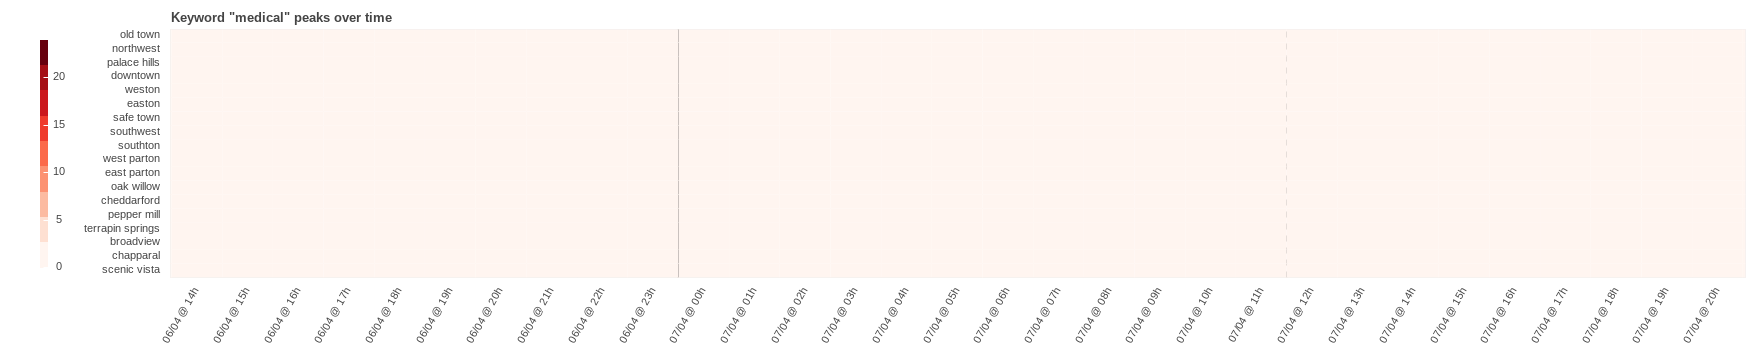
\includegraphics[width=1.00\textwidth]{figs/cond_30h/cond_30h_medical.png}
        \caption{Medical}
        \label{fig:medical_30h}
    \end{subfigure}
    \begin{subfigure}[!h]{0.24\textwidth}
        \centering
        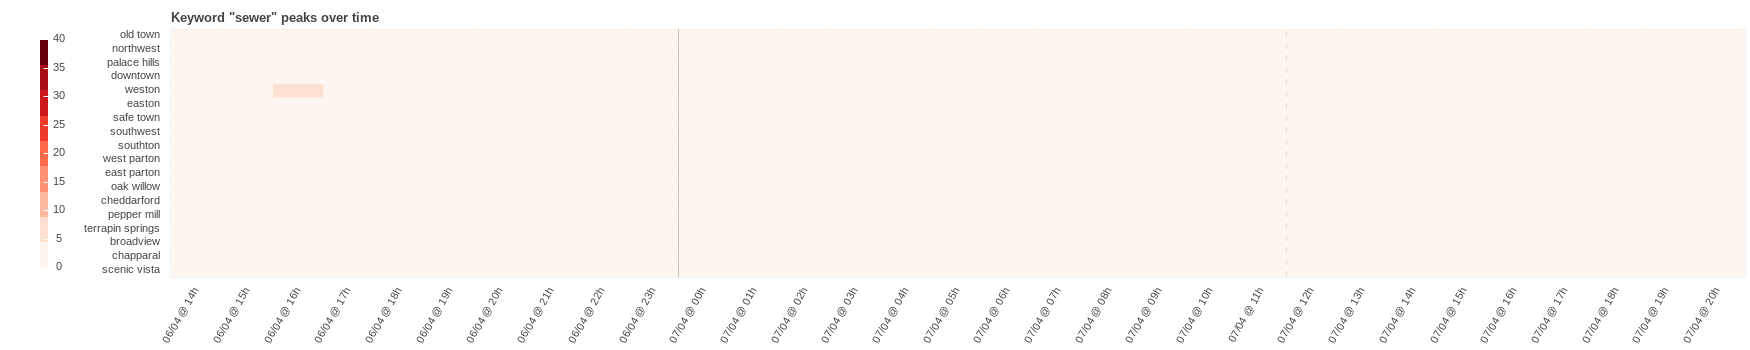
\includegraphics[width=1.00\textwidth]{figs/cond_30h/cond_30h_sewer.png}
        \caption{Sewer and water}
        \label{fig:sewer_30h}
    \end{subfigure}
    \begin{subfigure}[!h]{0.24\textwidth}
        \centering
        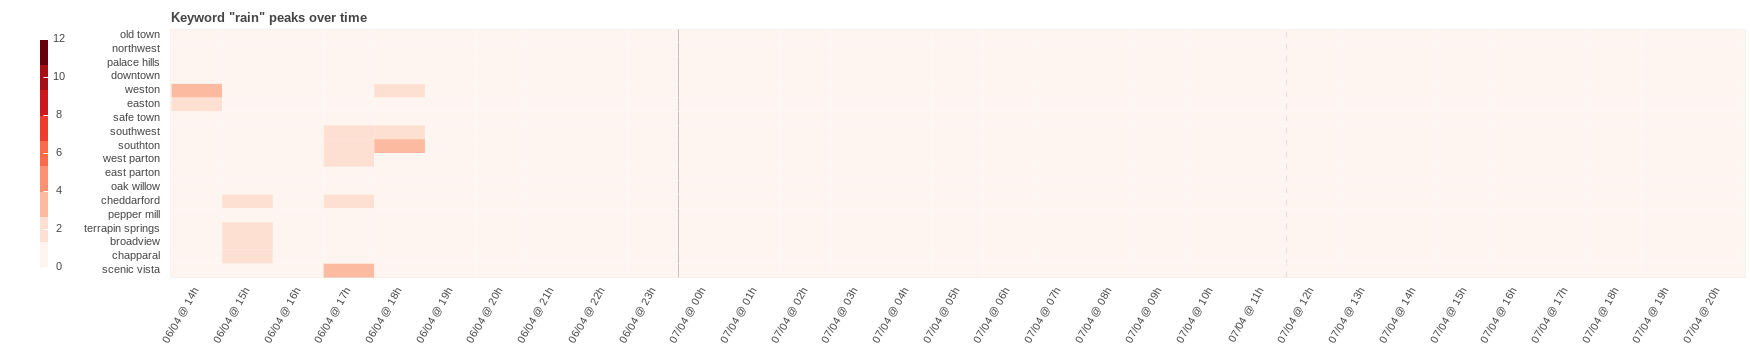
\includegraphics[width=1.00\textwidth]{figs/cond_30h/cond_30h_rain.png}
        \caption{Rain}
        \label{fig:rain_30h}
    \end{subfigure}
    \begin{subfigure}[!h]{0.24\textwidth}
        \centering
        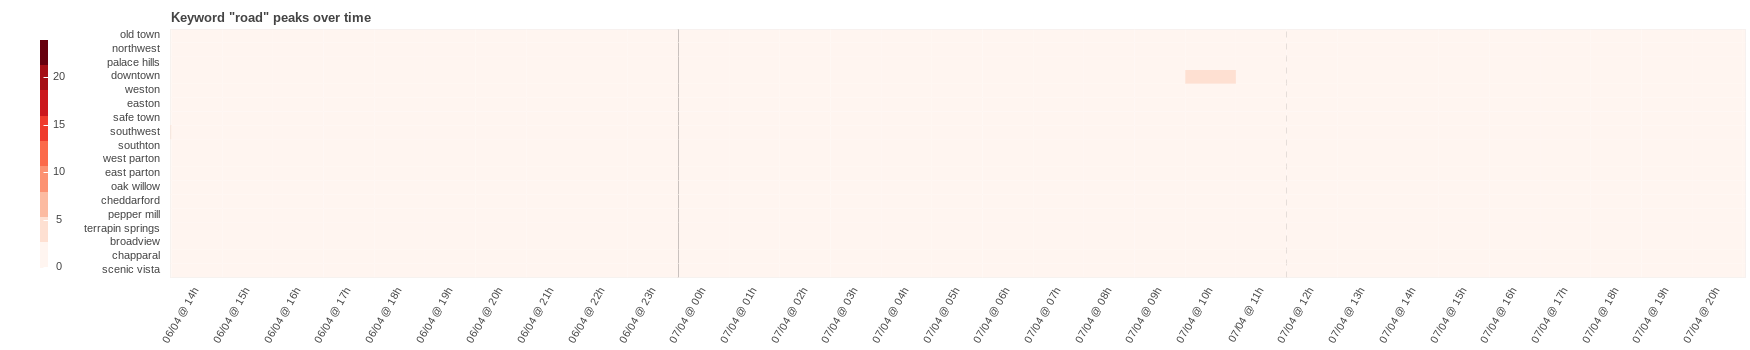
\includegraphics[width=1.00\textwidth]{figs/cond_30h/cond_30h_road.png}
        \caption{Roads and Bridges}
        \label{fig:roads_30h}
    \end{subfigure}
    \begin{subfigure}[!h]{0.98\textwidth}
        \centering
        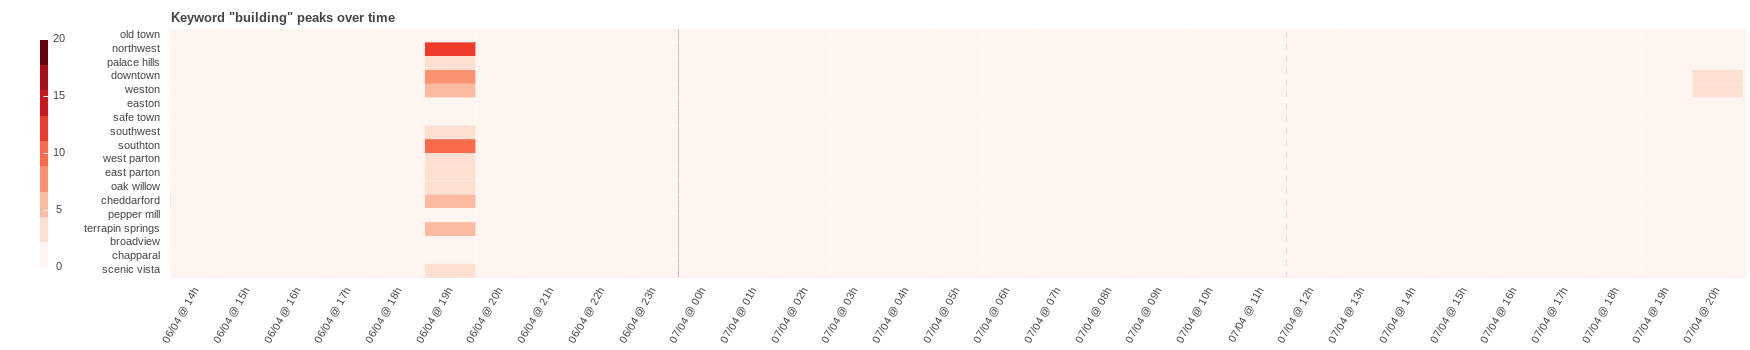
\includegraphics[width=1.00\textwidth]{figs/cond_30h/cond_30h_build.png}
        \caption{Building}
        \label{fig:building_30h}
    \end{subfigure}
    \begin{subfigure}[!h]{0.98\textwidth}
        \centering
        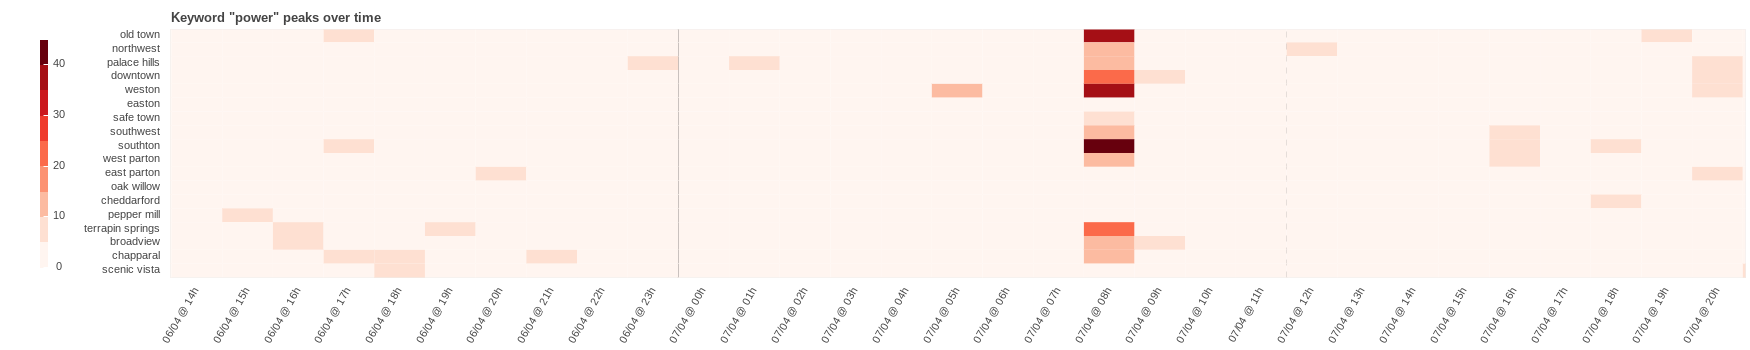
\includegraphics[width=1.00\textwidth]{figs/cond_30h/cond_30h_power.png}
        \caption{Power}
        \label{fig:power_30h}
    \end{subfigure}
    \caption{Conditions after 30h of the first earthquake}
    \label{fig:eq_cond_30h}
\end{figure}

By looking at the heatmap of Figure~\ref{fig:eq_cond_30h} for each keyword, it
can be seen that there have been no occurrences for medical, and the ones
related to sewer/water and rain have already been attended within the first five
hours. With respect to roads and bridges in particular, there have been 3
occurrences from 10:00~AM to 11:00~AM of April 8th at Downtown, but this
neighbourhood is under resurfacing maintenance, which implies a road crew is
already working there.

Suggestions for crew allocation is detailed as follows:

\begin{itemize}
    \item \emph{Building}: On April 7th from 7:00~PM to 7:59~PM there have been
    multiple casualties on almost all locations so we would prioritize the
    dark-red-colored ones according to the heatmap of
    Figure~\ref{fig:building_30h}:
    Northwest, Southton, Downtown, and Weston. All four have a high 
    density of buildings and people, apart from being geographically close to
    each other, which can be an advantage for an eventual reallocation of crews
    in the following hours. Terrapin Springs and Cheddarford also have some
    less-intense occurrences, but they must be ignored due to the absence of
    high buildings.
    \item \emph{Power}: According to Figure~\ref{fig:power_30h} on April 7th 
    there have been sporadic, less-intense
    occurrences that could be solved by sending small units to individual
    locations, but from 8:00~AM to 9:00~AM an energy disaster appear to have
    affected almost all neighbourhoods. Again we would prioritize regions where
    the keywords were mentioned the most: Southton, Old Town, and Weston. The
    other can be later attended in the following hours.
\end{itemize}
%%% EOF %%%

    \newpage

    \stepcounter{section}
    \section*{\tiny} % question 2
    \item \textcolor{gray}{Identify at least 3 times when conditions change in
        a way that warrants a re-allocation of city resources. What were the
        conditions before and after the inflection point? What locations were
        affected? Which resources are involved? Limit your response to 1000
        words and 10 images.}

    As already mentioned, there have been 3 independent earthquakes, as could be 
seen in Figure~\ref{fig:eq_start_heat}: Apr 6th 2:00~PM, Apr 8th 7:00~AM and Apr 
9th 3:00~PM, approximately. Those two last earthquakes are emphasized in
Figure~\ref{fig:eq_2_3_heat}.

\begin{figure}[!h]
    \centering
    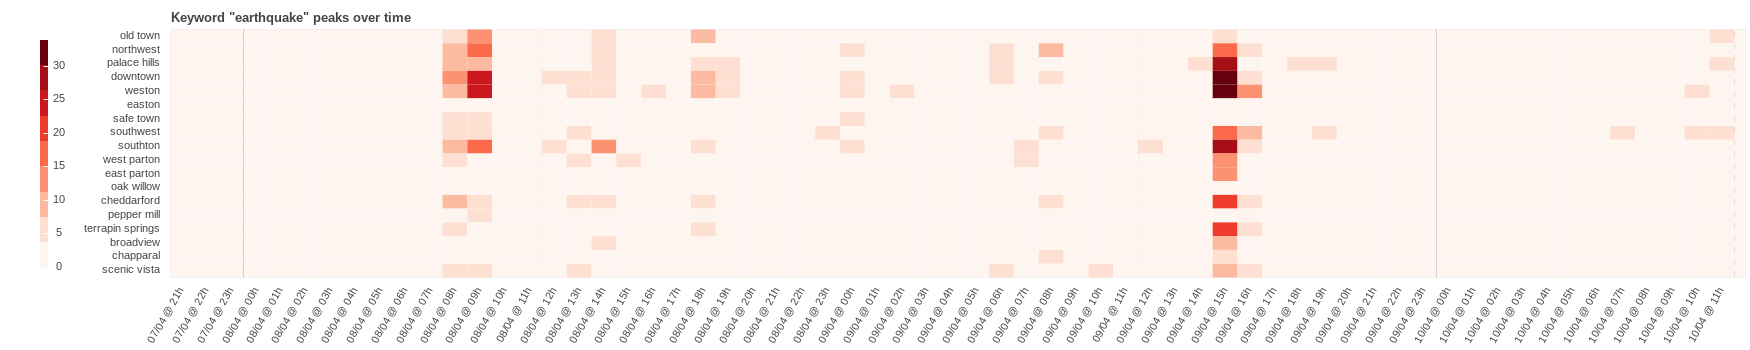
\includegraphics[width=1.00\textwidth]{figs/q2/eq_2_3_heat}
    \caption{Heatmap for the two last earquakes using keywords related to the
    word ``earthquake''.}
    \label{fig:eq_2_3_heat}
\end{figure}

\begin{figure}[!h]
    \centering
    \begin{subfigure}[!h]{0.96\textwidth}
        \centering
        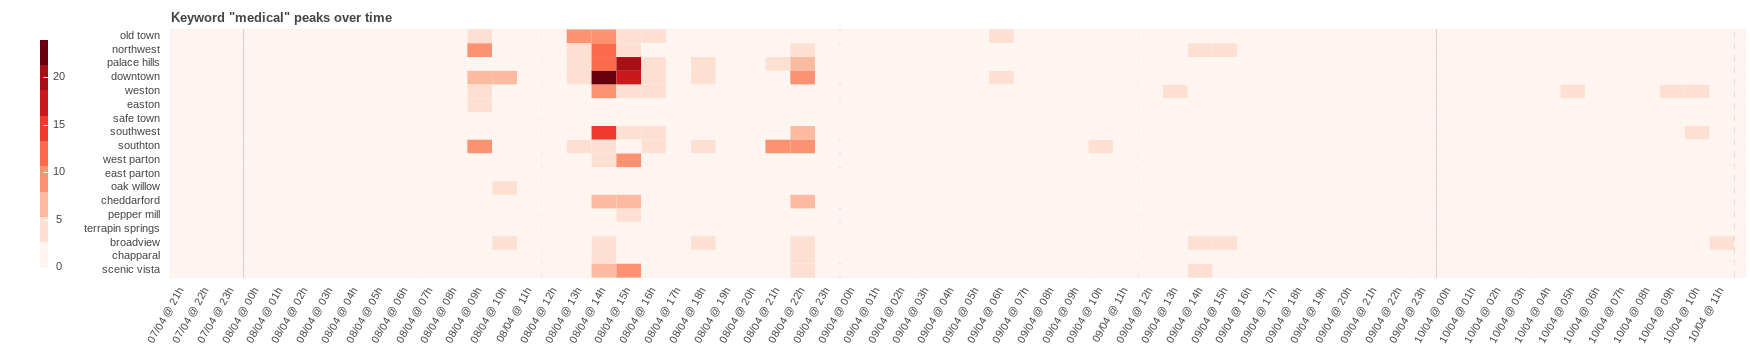
\includegraphics[width=1.00\textwidth]{figs/q2/medical_2_3_heat.png}
        \caption{Medical}
        \label{fig:medical_2_3_heat}
    \end{subfigure}
    \begin{subfigure}[!h]{0.96\textwidth}
        \centering
        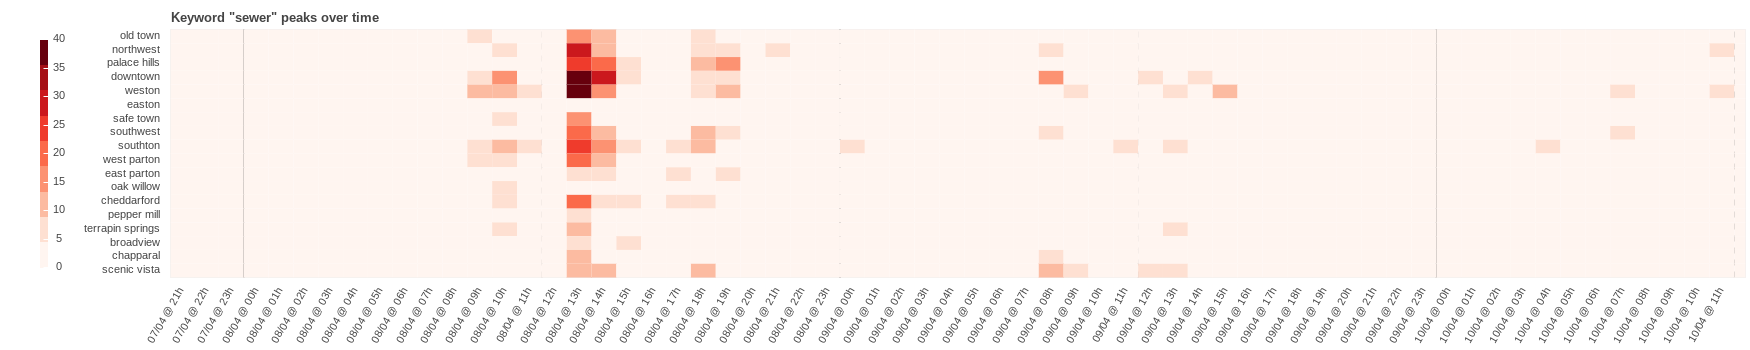
\includegraphics[width=1.00\textwidth]{figs/q2/sewer_2_3_heat.png}
        \caption{Sewer and water}
        \label{fig:sewer_2_3_heat}
    \end{subfigure}
    \begin{subfigure}[!h]{0.96\textwidth}
        \centering
        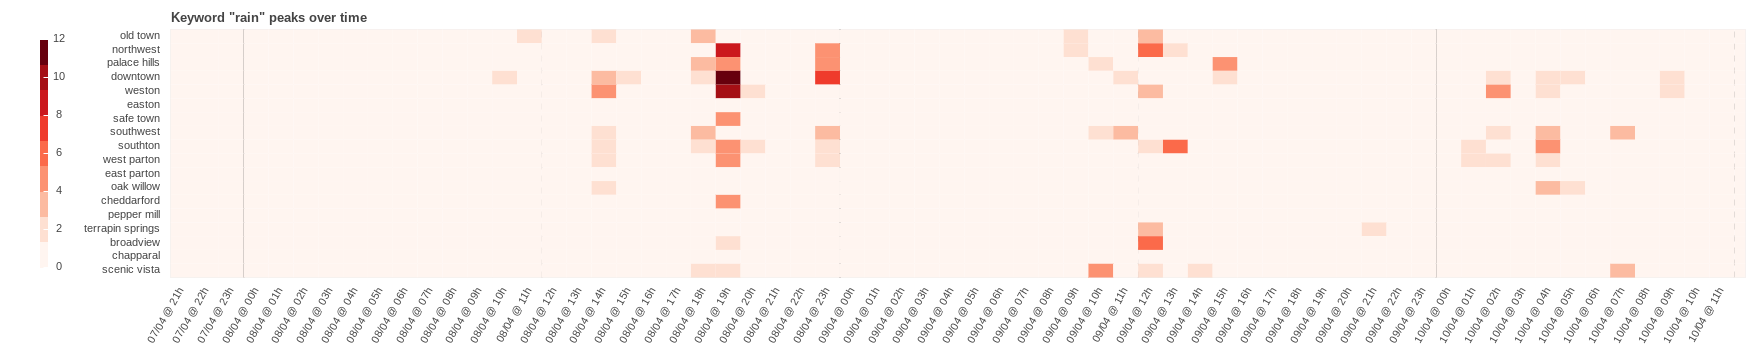
\includegraphics[width=1.00\textwidth]{figs/q2/rain_2_3_heat.png}
        \caption{Rain}
        \label{fig:rain_2_3_heat}
    \end{subfigure}
    \begin{subfigure}[!h]{0.96\textwidth}
        \centering
        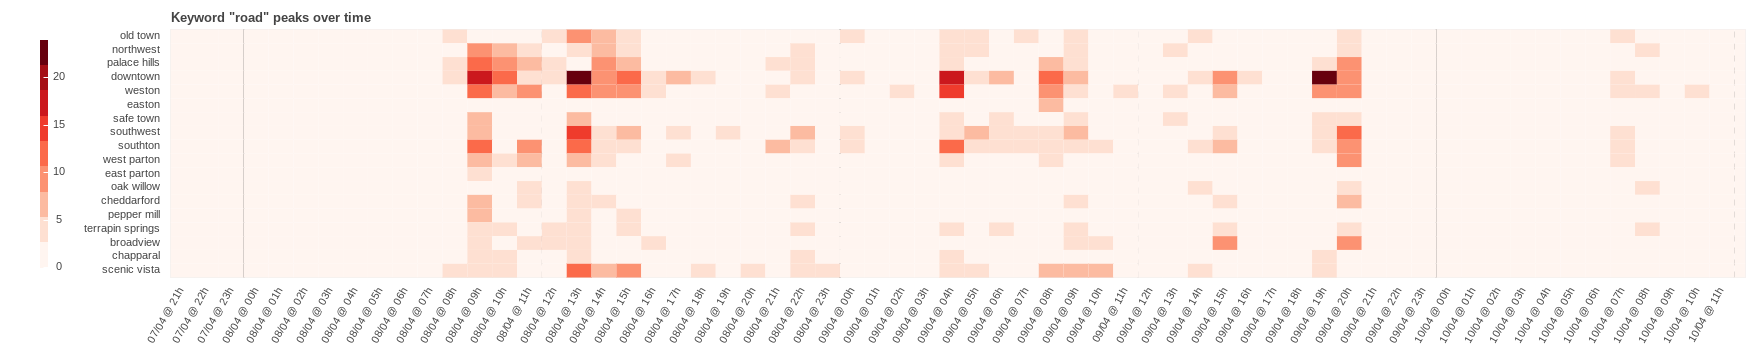
\includegraphics[width=1.00\textwidth]{figs/q2/road_2_3_heat.png}
        \caption{Roads and Bridges}
        \label{fig:roads_2_3_heat}
    \end{subfigure}
    \begin{subfigure}[!h]{0.96\textwidth}
        \centering
        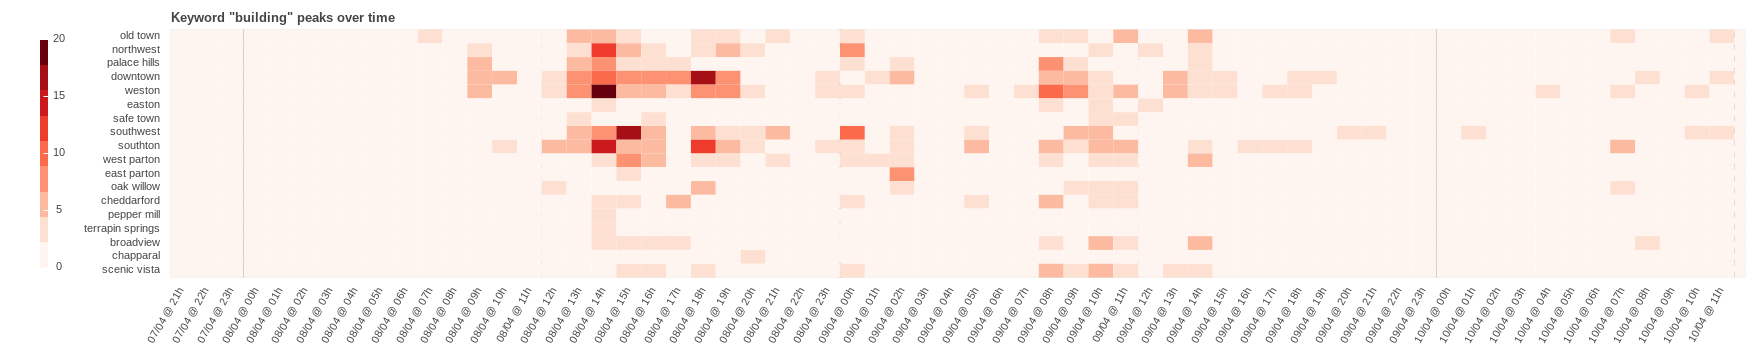
\includegraphics[width=1.00\textwidth]{figs/q2/build_2_3_heat.png}
        \caption{Building}
        \label{fig:building_2_3_heat}
    \end{subfigure}
    \begin{subfigure}[!h]{0.96\textwidth}
        \centering
        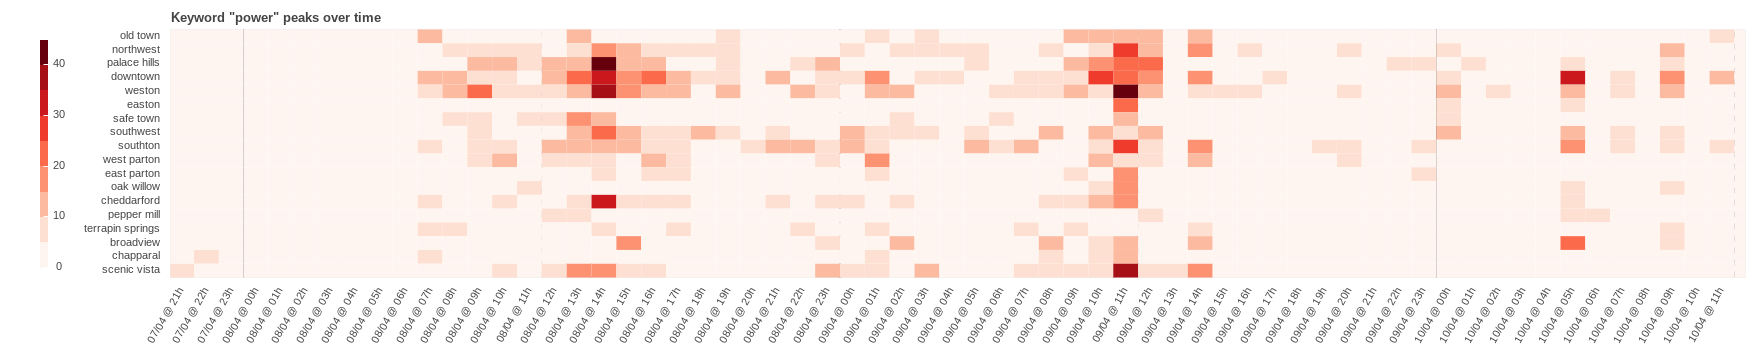
\includegraphics[width=1.00\textwidth]{figs/q2/power_2_3_heat.png}
        \caption{Power}
        \label{fig:power_2_3_heat}
    \end{subfigure}
    \caption{Heatmap of conditions for the two last earthquakes}
    \label{fig:eq_cond_2_3_heat}
\end{figure}

By looking at the heatmap of Figure~\ref{fig:eq_cond_2_3_heat} for each
keyword, it can be seen that the damaged inflicted by the
second earthquake was greater than both first and second ones.

Suggestions for re-allocation of city resources are detailed as follows:   

\begin{itemize}                                                                  
     \item \emph{Medical:} At least 12 hours before 9:00 AM of April 8th, there was no ocurrances regarding
medical keywords. On April 8th from 9:00 PM to 10:59 PM, the second earthquake
time, there have been casualties on multiple locations
but we would prioritize the darker colored ones according to the heatmap of Figure 8a:
Northwest, Southton and Downtown. First, a rescue crew must be sent to Northwest
and Southton between     
     9:00~AM and 9:59~AM. Then, from 9:00~AM and 9:59~AM, for being geographically close a crew must be realocated to
Downtown. 

Again, between 12:00 PM and 13:00 PM there have been no medical ocurrances but from 13:00 PM
to 16:00 PM, the number of ocurrances increased significantly and affected
almost all neighbourhoods except Safetown and Terrapin Springs. Accordingly, we
would prioritize the dark-red-colored ones, Downtown and Palace Hills, sending
rescue team from 14:00~PM and 15:00~PM for both neighbourhoods.  

On following hours after that peak in ocurrances, there have been only sporadic
requests that could be solved by sending small units to individual locations. 
\item \emph{Sewer and water:} A crew must be sent only to Weston between 4:00~PM and 4:59~PM.                                                          
     \smallskip                                                                   
     \item \emph{rain}: Issues have occurred in Pepper Mill, \textbf{Terrapin    
     Springs}, \textbf{Broadview}, Chapparal, \textbf{Southton}, \textbf{Old      
     Town} and Scenic Vista, but we'll consider only the locations                
     highlighted in bold because they have hospitals.                             
     \begin{itemize}                                                              
         \item A crew must be sent to Terrapin Springs between 3:00~PM and        
         3:59~PM. Broadview also has a power demand at this time interval but the 
         tweet frequency is much lower considering the five-hour period.                           \item Two crews must be sent to Old Town and Southton between 4:00~PM    
         and 4:59~PM.                                                             
         \item Lastly, the crew from Terrapin Springs can be reallocated to                Chapparal between 5:00~PM and 5:59~PM. Although Chapparal does not have  
         hospitals, it has been nearly two hours with electrical issues.          
     \end{itemize}                                                                
     \item \emph{R}: A crew must be sent to Southton only   
     because there have been small issues in Weston, Southton and Downtown, and   
     therefore Southton is geographically in the middle of such neighbourhoods.   
 \end{itemize}   

\begin{figure}[!h]
    \centering
    \begin{subfigure}[!h]{0.98\textwidth}
        \centering
        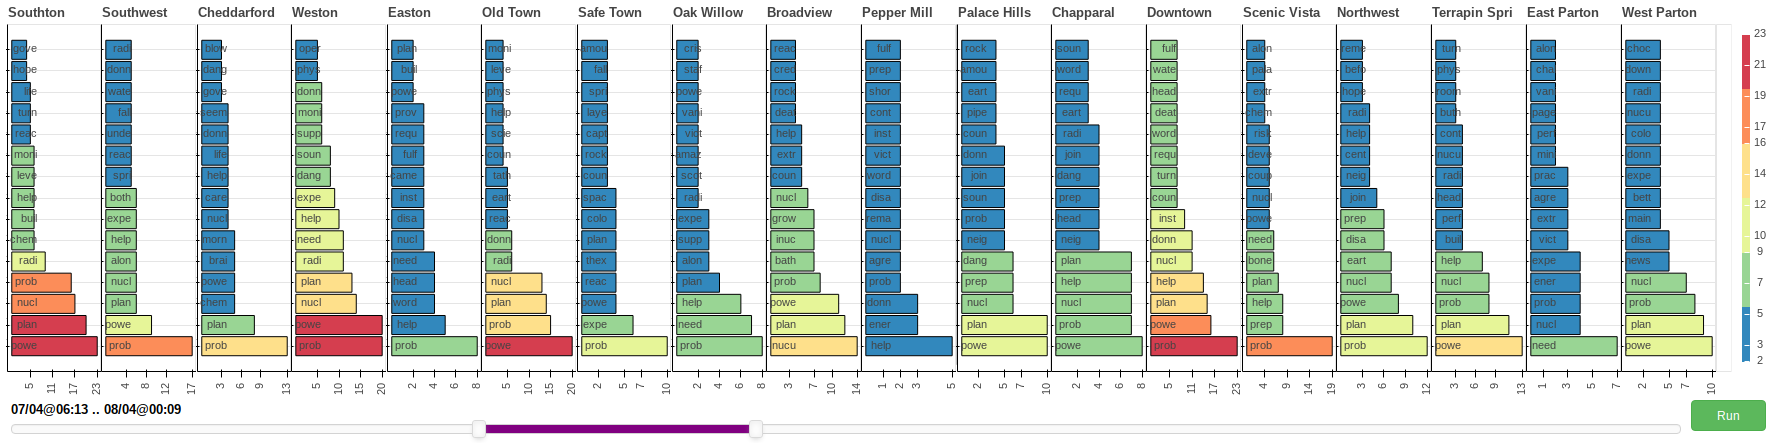
\includegraphics[width=1.00\textwidth]{figs/q2/eq_2_hbar.png}
        \caption{Bar chart for the second earthquake in a 18h time interval from
        Apr 7th at 6:00~PM to Apr 8th at 12:00~AM.}
        \label{fig:eq_2_hbar}
    \end{subfigure}
    \begin{subfigure}[!h]{0.98\textwidth}
        \centering
        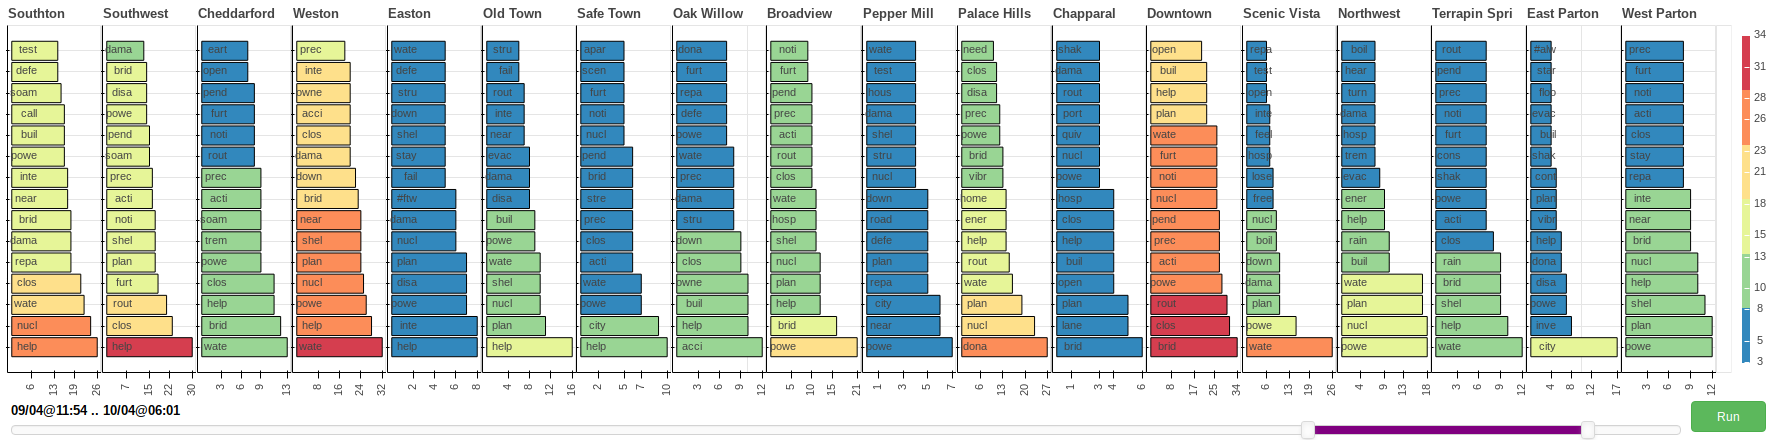
\includegraphics[width=1.00\textwidth]{figs/q2/eq_3_hbar.png}
        \caption{Bar chart for the third earthquake in a 18h time interval from
        Apr 9th at 12:00~PM to Apr 10th at 6:00~AM.}
        \label{fig:eq_3_hbar}
    \end{subfigure}
    \caption{eae}
    \label{fig:eq_2_3_hbar}
\end{figure}

\begin{figure}[!h]
    \centering
    \begin{subfigure}[!h]{0.46\textwidth}
        \centering
        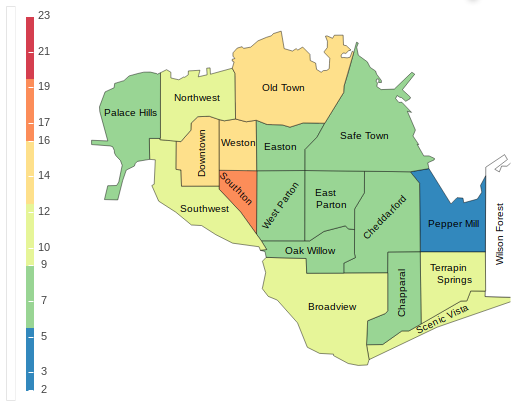
\includegraphics[width=1.00\textwidth]{figs/q2/eq_2_svg.png}
        \caption{Map for the second earthquake. Yellow and orange shades show
        locations where the frequency of tweets is higher. Southton, Downtown,
        Weston and Old Town appear to be, in that order, the neighbourhoods that 
        most need help.}
        \label{fig:eq_2_svg}
    \end{subfigure}
    \hspace{0.75cm}
    \begin{subfigure}[!h]{0.46\textwidth}
        \centering
        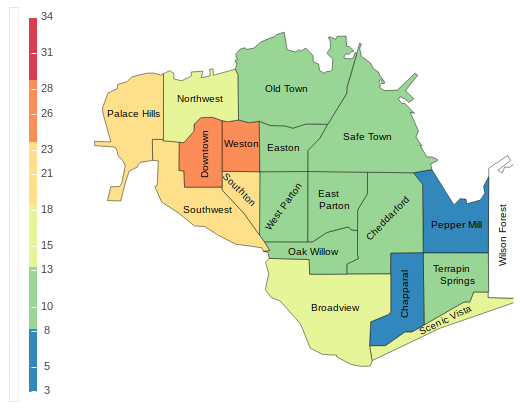
\includegraphics[width=1.00\textwidth]{figs/q2/eq_3_svg.png}
        \caption{Map for the third earthquake. Yellow and orange shades show
        locations where the frequency of tweets is higher. Downtown, Weston,
        Pallace Hills, Southwest, and Southton appear to be, in that order, the 
        neighbourhoods that most need help.}
        \label{fig:eq_3_svg}
    \end{subfigure}
    \caption{St. Himark's SVG maps with blue-to-red colormap for the second and
    third earthquakes.}
    \label{fig:eq_2_3_svg}
\end{figure}


    \newpage

    \stepcounter{section}
    \section*{\tiny} % question 3
    \item \textcolor{gray}{Take the pulse of the community.  How has the
        earthquake affected life in St. Himark? What is the community
        experiencing outside the realm of the first two questions? Show decision
        makers summary information and relevant/characteristic examples. Limit
        your response to 800 words and 8 images.}

    pay no cy da birguesia

    \newpage

    \stepcounter{section}
    \section*{\tiny} % question 4
    \item \textcolor{gray}{The data for this challenge can be analyzed either as
        a static collection or as a dynamic stream of data, as it would occur in
        a real emergency. Describe how you analyzed the data --- as a static
        collection or a stream. How do you think this choice affected your
        analysis? Limit your response to 200 words and 3 images.}

    The data were analyzed as static collection in order to facilitate
interpretation of the problems. Using a stream analysis many decision-making
for the allocation of resources might be misleading.
Figure~\ref{fig:rain_4_heat} shows an example for the keyword \emph{``rain''}.

\begin{figure}[!h]
    \centering
    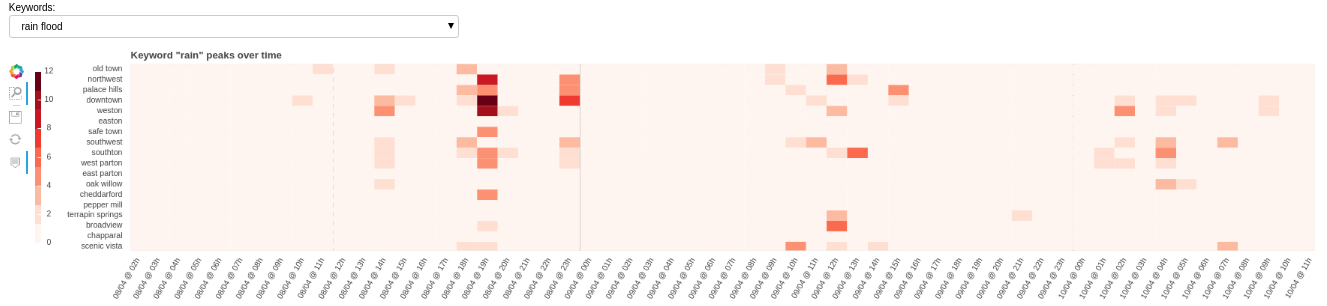
\includegraphics[width=1.00\textwidth]{figs/q4/rain_4_heat}
    \caption{Heatmap for the ``\emph{rain}''.}
    \label{fig:rain_4_heat}
\end{figure}

At 6:00 PM, five neighborhoods tweeted about rain or flood. If for each locality
a rescue team was sent, at 7:00 PM where almost all localities reported rain or
flood occurrences, so it would have been more difficult to efficiently serve all
those affected neighborhoods.

\end{enumerate}
\end{document}
